\documentclass[a4paper,12pt]{article}
\usepackage[utf8]{inputenc}
\usepackage[T1]{fontenc}
\usepackage[spanish]{babel}
\usepackage{csquotes}
\usepackage{anysize}
\usepackage{graphicx}
\marginsize{25mm}{25mm}{25mm}{25mm}

\title{Prior knowledge on the illumination position}
\author{Pascal Mamassian \and Ross Goutcher}
\date{2001}

\begin{document}
{\scshape\bfseries \maketitle}

La percepción visual es ambigua dado que infinitas escenas son compatibles con la misma impresión retinal. A pesar de ello experimentamos solamente un percepto estable, robusto y unitario. Para lidiar con la ambigüedad el sistema visual debe utilizar conocimiento extra-retinal {\itshape a priori}.

Un conocimiento frecuentemente citado es la presunción de que la luz viene de encima del observador. El primer reporte de este fenómeno se encontró en 1744: un sello mirado a través de un tubo óptico o un microscopio se veía convexo en sus partes cóncavas y viceversa. El fenómeno se debió a que la imagen vista a través del tubo se encontraba de cabeza, por lo que las sombras estaban en el lugar incorrecto relativas a la fuente de luz: las sombras eran consistentes con un objeto cuyo relieve esta invertido.

Experimentos han mostrado que este supuesto de la fuente de iluminación depende de la posición de la cabeza del observador y no de la gravedad. Curiosamente, se ha observado un sesgo consistente en esta presunción, con lo que los participantes suelen suponer que la luz proviene de arriba y levemente de la izquierda de su posición.

La idea de que la luz venga de arriba a la izquierda es inesperada dado que  las presunciones suelen estar relacionadas con regularidades estadísticas del ambiente. Es contraintuitivo que los humanos pasen más tiempo con la luz viniendo de arriba a su izquierda que de su derecha. Una explicación es que los observadores, al manipular objetos, se colocan con la luz viniendo de su izquierda mientras manipulan el objeto con la mano derecha. Esto anticiparía una relación entre este sesgo y la dominancia de las manos. Tal relación ha sido encontrada.

Sin embargo, la evidencia a favor de la existencia de este sesgo no es del todo sólida. Este experimento busca aportar evidencia más sistemática.

{\scshape\bfseries Experiment}

Se usan estímulos cuya interpretación cambia con la posición de la iluminación. No se usan esferas debido a que existe un sesgo distinto para percibir objetos convexos por encima de cóncavos.

Se usan estímulos que representan superficies planas con tiras paralelas sobresalientes. Cuando la fuente de luz se mueve de arriba hacia abajo el percepto cambia de tiras angostas sobresalientes a barras gruesas sobresalientes (figura 1).

\begin{figure}[ht]
	\begin{center}
		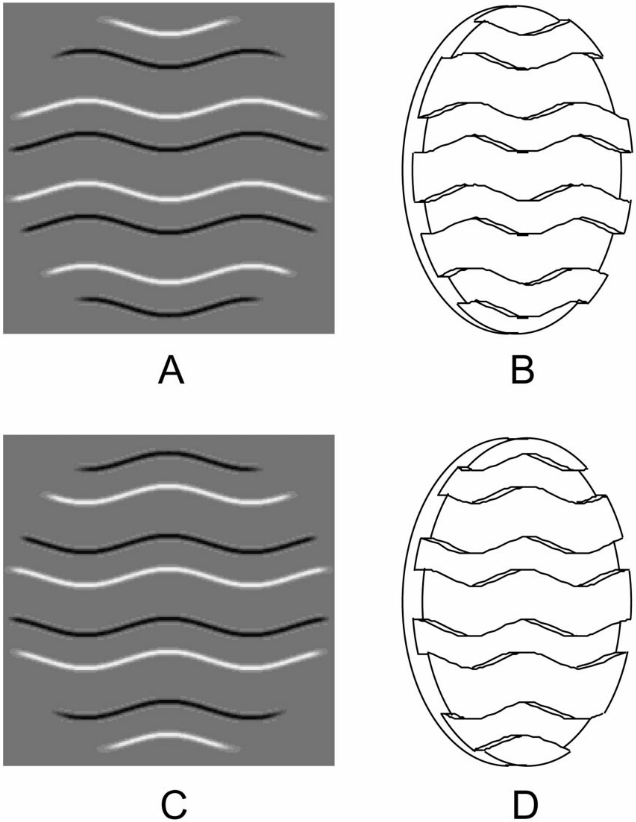
\includegraphics[scale=0.4]{Mamassian2001(1).png}
		\caption{Ejemplos de estímulos utilizados en la tarea (A, C) y su interpretación típica (B, D).}
	\end{center}	
\end{figure}

Los estímulos se presentan en varias orientaciones, con lo que se rota a la vez la superficie y la fuente de luz. Se asume que la orientación de la superficie es irrelevante, por lo que toda diferencia se atribuirá a la dirección de la luz. Se hipotetiza que la posición de iluminación que más consistentemente produzca el percepto de ``tiras angostas'' será la posición asumida por el observador.

{\scshape\bfseries Method}

Cada patrón tenía dos variantes de modo que el punto de fijación cayera tanto en tiras angostas como en tiras anchas. Esta manipulación no produjo ninguna diferencia en los resultados. Cada patrón se presentó en 24 orientaciones en el plano en incrementos de 15 grados.

Se probó la dominancia manual de los participantes. Se incluyeron 10 zurdos y 10 diestros.

Se presentaron a los participantes dos bloques de ensayos consistentes en un punto de fijación seguido de una figura en una orientación aleatoria seguida de una imagen de ruido blanco. Las imágenes se presentaron por 120 ms, lo que evitaba las reversiones en el percepto que ocurren con tiempos de exposición largos. La tarea de los observadores era reportar si las tiras que aparecían sobresalir en la imagen eran agostas o anchas. Respondían con las teclas de un teclado y no se daba realimentación. Cada orientación se presentó 16 veces. Se nombró {\itshape narrow score} a la proporción de ocasiones que un estímulo fue interpretado como una superficie con tira angostas sobresalientes.

{\scshape\bfseries Results}

Los resultados se presentan en la figura 2. El eje X representa la orientación de los estímulos en el plano frontal, y el origen es la orientación del patrón de la figura 1A, y las orientaciones positivas van en contra de la dirección del reloj. La posición de la iluminación asumida por el observador se puede inferir de la orientación del estímulo que lleva a un pico en el {\itshape narrow score}. Si la luz viniese directamente de arriba el pico se encontraría en el centro de la gráfica. En lugar de ello el pico se encuentra a la derecha, lo que indica que la posición preferida de iluminación está a la izquierda de la vertical.

\begin{figure}[ht]
	\begin{center}
		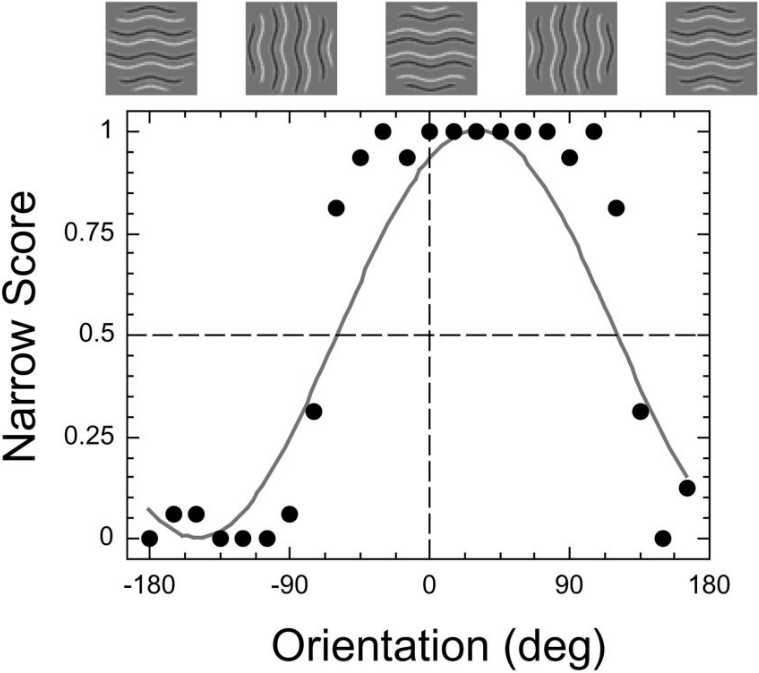
\includegraphics[scale=0.4]{Mamassian2001(2).png}
		\caption{Variación del {\itshape narrow score} en función de la orientación para un observador representativo.}
	\end{center}
\end{figure}

Se computó la posición preferida para cada observador.

Cuatro participantes (tres zurdos, uno diestro) fueron descartados dado que ejecutaron a nivel del azar. Con los restantes se realizó una regresión lineal del sesgo de posición de iluminación contra la dominancia manual. También se realizó un análisis no paramétrico de Mann-Whitney para comparar la media de la posición del sesgo entre los dos grupos. En ningún caso se encontró una diferencia.

{\scshape\bfseries Discussion}

La existencia de ilusiones como la ilusión del cráter ha sido tomada como evidencia de la habilidad del sistema visual para tomar en cuenta regularidades salientes del ambiente. Saber el origen de la luz puede resolver la ambigüedad y acelerar la interpretación de escenas naturales.

Este experimento confirma hallazgos previos que indicaban que la posición preferida de iluminación está sesgada hacia arriba a la izquierda en lugar de directamente arriba. Este sesgo es, en promedio, de 26°, y es de magnitud similar en zurdos y diestros. Es difícil dar una explicación ecológica de este sesgo debido a que los humanos tienden a estar expuestos a múltiples fuentes de iluminación, a iluminación difusa, y rara vez se encuentran directamente bajo el sol. Y aún entonces, sería difícil probar que se orientan más a menudo con la luz en su lado izquierdo.

El origen de los resultados puede ser un sesgo en el campo visual: hay evidencia que indica que los observadores prestan más atención al lado derecho de una cara (en el hemicampo derecho del observador) cuando intentan identificar el género. El lado derecho de la cara será informativo solo si la luz está a la izquierda del observador. Una preferencia para atender a un lado de los objetos podría estar relacionada con un sesgo en la posición de la iluminación. Esto anticipa que pacientes con lesiones parietales derechas (que ignoran el lado izquierdo de los objetos) podrían asumir que la iluminación proviene de una localización distinta.

La relación entre lateralización cerebral y la posición de la iluminación podría explicar la discrepancia con los resultados de autores que encontraron una correlación entre la dominancia manual y el sesgo de la posición de la iluminación: hay una gran variabilidad en la lateralización cerebral de los zurdos. Es posible que la población surda de ese estudio incluyera a varios participantes con una dominancia cerebral izquierda.

Si esta lateralización es el origen del sesgo, se podría esperar encontrarla en la vida temprana. Se ha encontrado evidencia a favor de esta interpretación en estudios con pollos criados en un ambiente en el cual la luz provenía desde abajo, pero que aún así se comportaban como si viniese desde arriba. Es posible que estas presunciones {\itshape a priori} se encuentren representadas cerebralmente y que un mecanismo genético se encargue de la herencia de este conocimiento.


\end{document}
